\chapter{Analíticas de Elasticsearch y Dash}
\label{analiticas}
En este capítulo se explica la recogida de las sondas en Unibotics, su posterior guardado en la base de datos Elasticsearch, la visualización de dichos datos con el \textit{framework} web Dash y la validación experimental del proceso.
\section{Recogida de sondas}
La primera parte de este proceso ha consistido en la recogida de diferentes sondas. Para realizar esta tarea, se ha decidido utilizar la herramienta de Elasticsearch por las ventajas que ofrece explicadas en el capitulo 3.\\

En este proyecto se ha utilizado Docker, un contenedor a nivel de sistema operativo para Elasticsearch. Se ha utilizado Docker debido que permite que Elasticsearch funcione en cualquier sistema operativo, y replicar la instalación en cualquier máquina es directo. Primero hay que descargar la imagen de Elasticsearch con la versión deseada en este caso se ha utilizado la 7.12.0, el comando para descargar la imagen es:
{\footnotesize
		\begin{verbatim}
			docker pull docker.elastic.co/elasticsearch/elasticsearch:7.12.0
		\end{verbatim}
		}
        
Para ejecutar el contenedor con la imagen descargada se utiliza el siguiente comando:

{\footnotesize
		\begin{verbatim}
			docker run --name=AcademyElastic -p 9200:9200 -p 9300:9300
            -e "discovery.type=single-node" 
            docker.elastic.co/elasticsearch/elasticsearch:7.12.0
		\end{verbatim}
		}
   \newpage   
  Una vez ya puesto en marcha el contenedor de Elasticsearch ya tenemos nuestra base de datos donde se guardaran las sondas. Para hacer solicitudes se podrá hacer mediante \textit{REST APIs}, un ejemplo sería introducir en el navegador la siguiente URL: \texttt{http://localhost:9200/}.\\
  
  El siguiente paso es la integración de Elasticseach en el servidor basado en Django. Para ello se hará uso de la librería \texttt{django-elasticsearch-dsl}. Además se ha modificado el archivo de configuración del proyecto, \texttt{settings.py},  añadiendo la librería a las aplicaciones instaladas y creando una nueva variable llamada \texttt{ELASTICSEARCH\_DSL}, también en \texttt{settings.py}, ya que las variables declaradas en ese fichero se pueden utilizar en cualquier parte del servidor. En esa variable se indica el servidor de Elasticsearch con el que se tiene que conectar y sincronizar.\\
  
Una vez conectado Django con Elasticsearch se han definido y configurado los índices donde se guardaran las sondas, para ellos se ha creado un nuevo archivo llamado \texttt{probe.py}. Al definir un índice, se determinan los nombres de cada campo (información que se quiere almacenar) con el tipo de campo que es, por ejemplo si es un texto, un número, una fecha, entre otros. También se puede configurar el índice, por ejemplo poniendo el número de\textit{ shards }o el número de réplicas. Un ejemplo de la definición de un índice sería este: 

\begin{lstlisting}
   from django_elasticsearch_dsl import Document, Date, Text, Double
   
   class SessionDocument(Document):
    		username = Text()
  	  		start_date = Date()
   			end_date = Date()
    		duration = Double()
    		client_ip = Text()
    		browser = Text()
    		country = Text()
    		alpha_2 = Text()
    		alpha_3 = Text()
    		continent = Text()
    		class Index:
        		name = 'session_log'
        		settings = {
            			'number_of_shards': 1,
           				'number_of_replicas': 0
        }
\end{lstlisting} 

Para este proyecto se han definido cuatro índices diferentes:

\begin{itemize}
\item \texttt{session\_log}: índice que recoge las sondas relativos a las sesiones. Consta de los campos de inicio y fin de sesión, duración de la sesión, la IP, el \textit{browser} (aporta información sobre el sistema operativo, navegador y dispositivo utilizado), el continente y país del usuario, así como el nombre del usuario.
\item \texttt{exercises\_log}: índice que recoge las sondas relativos a los diferentes ejercicios. Esta compuesto por la fecha de entrada en un ejercicio, la fecha de salida del ejercicio, la duración total, el nombre del ejercicio y el usuario.
\item \texttt{style\_log}: índice que recoge los datos sobre la evaluación del estilo del código de los ejercicios. Este índice esta formado por el campo de la fecha en la que se realiza la evaluación, el nombre del ejercicio, la puntuación sobre 100 y el nombre del usuario.
\item \texttt{efficacy\_log}: índice que recoge los datos sobre la evaluación de la eficacia del código de los ejercicios. Los campos son iguales que en el índice de \texttt{style\_log}.
\end{itemize}

Ya definidos los diferentes índices se importan al archivo \texttt{views.py} para poder crearlos. Las sesiones de los usuarios se guardan en el índice \texttt{session\_log} y a través de las sondas creadas, por ello podemos recoger cuando el usuario \textit{loguea} en la plataforma y cuando finaliza su actividad en ella. Se recoge la sonda de la siguiente manera:
\\
{\footnotesize
\begin{verbatim}
    probe_session = SessionDocument(username=username,start_date=datetime.now(),
                                    end_date=datetime.now(),duration=0, client_ip=ip,
                                    browser=request.META['HTTP_USER_AGENT'],
                                    country=location_info["country_name"],
                                    alpha_2=location_info["alpha_2"], 
                                    alpha_3=location_info["alpha_3"],
                                    continent=location_info["continent"])
    probe_session.save()
\end{verbatim}
}
\newpage
Gracias al objeto HTTP Request que recibe el fichero \texttt{views.py} obtenemos la información del nombre del usuario, la IP y el \textit{user-agent} el cual nos dirá el sistema operativo, el navegador o el dispositivo que utiliza el usuario. Para la localización se ha creado una función que a partir de la IP muestra la ubicación. Cuando el usuario \textit{loguea}, los campos  de fin de sesión y duración se inicializan con la fecha actual y 0 respectivamente, una vez que el usuario haga \textit{logout} o finalice su sesión por inactividad estos campos se modificarán como se muestra a continuación:\\
{\footnotesize
\begin{verbatim}
    s = Search(index="session_log").query('match', username=request.user.username) \
                                    .sort({"start_date": {'order':'desc'}})[0]
    for hit in s:
        end = datetime.now()
        Elasticsearch(settings.ELASTICSEARCH_DSL['default']['hosts']) \
                        .update(index="session_log", id=hit.meta.id,
                                body={"doc": {'end_date': end,
                                'duration':(end - datetime \
                                    .strptime(hit.start_date,'%Y%m%dT%H:%M:%S.%f')) \
                                    .total_seconds()}})
\end{verbatim}
}
\\
Las sondas relativas a los ejercicios se guardan cuando el usuario accede a un ejercicio y como ocurre con las sesiones, cuando el usuario abandone el ejercicio se modificarán los datos de duración y fin del ejercicio. Se ha tenido en cuenta que al recargar un ejercicio en el que el usuario ya se encontraba, no se cree una sonda nueva y se tenga en cuenta la primera sonda creada para dicho ejercicio. Las sondas no deseadas que se han creado se eliminan de la siguiente forma:\\
\\
{\footnotesize
\begin{verbatim}
   es = Search(index="exercises_log").query('match', duration=0)  \
   				            .query('match', username=request.user.username)  \
        					                .sort({"start_date": {'order':'desc'}})
    for hit in es:
        Elasticsearch(settings.ELASTICSEARCH_DSL['default']['hosts'])  \ 
    				                        .delete(index="exercises_log", id=hit.meta.id)
\end{verbatim}
}
\\
Cada ejercicio que se encuentra en Unibotics dispone de un botón de evaluación automática de estilo, donde se dan unas recomendaciones para mejorar el estilo del código del usuario con una puntuación. La puntuación es recogida en el índice de \texttt{style\_log}. Para poder recoger la puntuación recibida en la evaluación de eficacia, se ha creado un nuevo botón en los ejercicios. Una vez pulsado el botón, empieza a ejecutar el código durante un tiempo determinado según el ejercicio. Pasado ese tiempo se obtiene la nota obtenida del ejercicio y se guarda en el índice de \texttt{efficacy\_log}. Si el usuario pulsa dos veces al botón la sonda no se guardará.\\


En este proceso de recogida de sondas y su grabación ha sido muy útil la utilización de la API que proporciona Elasticsearch para poder depurar y comprobar los datos que se estaban almacenando. Utilizando por ejemplo la URL \texttt{http://127.0.0.1:9200/session\_log/\_search/?size=10000&pretty} se comprueba las sondas de sessiones.\\

Para comprobar el funcionamiento de Elasticsearch se generaron datos de prueba para poder comenzar a trabajar antes de tener los datos reales los cuales llevan tiempo recoger. La base de datos Elasticsearch dummy se ha creado gracias a las librerías de Python Faker\footnote{https://faker.readthedocs.io/en/master/} y Tornado\footnote{https://www.tornadoweb.org/en/stable/} en ella se puede modificar las sondas como por ejemplo el número de sondas, de réplicas o de \textit{shards}. Esto ayudará a futuros desarrolladores a utilizar la base de datos de Elasticsearch. En la Figura\ref{fig:dummy} se muestra como ejemplo el resultado de la sonda de evaluación de estilo de la base de datos de prueba.


\begin{figure}[H]
    \centering
    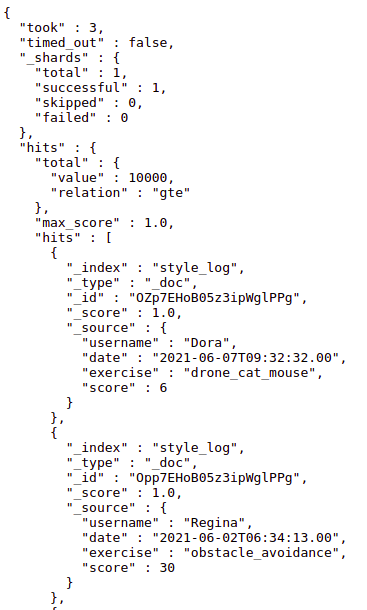
\includegraphics[width=5cm, keepaspectratio]{img/dummy.png}
    \caption{Elasticsearch dummy}
    \label{fig:dummy}
\end{figure}

\section{Visualización de la información}

Dash es un \textit{framework} web que permite crear tableros web interactivos con visualizaciones dinámicas, para poder hacer análisis como se explica en el capítulo 3. En este Trabajo de fin de grado se ha decidió utilizar esta herramienta para la visualización de las sondas recogidas en Elasticsearch.\\

Sólo los usuarios registrados en Unibotics podrán acceder a las visualizaciones y, dependiendo del tipo de usuario, tendrán disponibles unas visualizaciones u otras. Para iniciar sesión, se ha hecho uso de los usuarios ya guardados en la base de datos MYSQL de la que depende Django en la que se encuentra la información sobre el tipo de usuario (staff, admin, user...). En el caso de los administradores podrán ver la información de todas las sondas, mientras que un usuario de Unibotics solo podrá acceder a las puntuaciones de estilo y de eficacia obtenidas en cada ejercicio. En la Figura \ref{fig:menu} muestra el menú disponible para los administradores.

\begin{figure}[H]
    \centering
    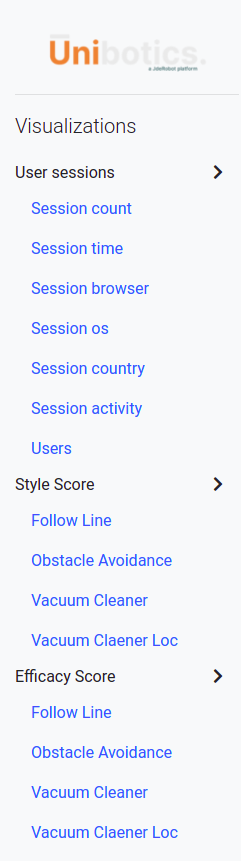
\includegraphics[width=3cm, keepaspectratio]{img/menu.png}
    \caption{Menú de un administrador en Dash}
    \label{fig:menu}
\end{figure}

\newpage
Gracias a las bibliotecas de Dash mencionadas en el capítulo 3 se ha dado estilo y formato a la aplicación, también se ha hecho uso de la \textit{cookies }del navegador para comprobar si se esta autorizado y si es un administrador de la plataforma.\\

Dash trabaja con dataframes, por lo que es necesario realizar una primera transformación de los datos de Elasticsearch a esta estructura, gracias a la biblioteca de Pandas. Un ejemplo de la realización de esta conversión es:

{\footnotesize
\begin{verbatim}
  s = Search(using=es, index="session_log")
  results = [hit.to_dict() for hit in s.scan()]
  df  = pd.DataFrame(results)
\end{verbatim}
}
\\

Con la biblioteca \texttt{dash\_core\_components} se han creado los filtros que algunas de las gráficas poseen. Estos filtros de forma dinámica cambian las visualizaciones en base a dicho filtrado. Uno de los filtros que más se utilizado es el filtro por fechas. Estableciendo una fecha de inicio o de fin o ambas es posible conocer la situación de Unibotics en un periodo de tiempo concreto. El código de filtrado ha sido:

{\footnotesize
\begin{verbatim}
 if start_date is not None and end_date is not None:
        df=df.loc[(df['start_date'] > start_date) & (df['start_date'] <= end_date)]
elif start_date is not None:
        df=df.loc[(df['start_date'] > start_date)]
elif end_date is not None:
        df=df.loc[(df['start_date'] <= end_date)]
\end{verbatim}
}
\\

Otro filtro recurrente en la mayoría de las visualizaciones es el filtro por usuario. Este filtro se encuentra, además en las gráficas de las evaluaciones de estilo y eficacia del código pero solo para los administradores, así podrán ver las puntuaciones de los diferentes usuarios. Para este filtro se hace uso de las sondas de sesiones, recogiendo los nombres de los usuarios de forma única y añadiendo un 'Total' en los casos que se quiera visualizar las sondas de todos los usuarios. En resumen el filtro podrá filtrar por usuario único, un grupo de usuarios o por el total de los usuarios, \texttt{df = df[df.username.isin(user)]} . El código para conseguir los nombre de los usuarios y añadir la opción de 'Total', es el siguiente:
\newpage
{\footnotesize
\begin{verbatim}
	s = Search(using=es, index="session_log")
    results = [hit.to_dict() for hit in s.scan()]
    df  = pd.DataFrame(results)
    df = df[df['username'].notna()]
    users = df['username'].unique()
    if not exercises:
        users = np.insert(users,0,'Total')
    return users
\end{verbatim}
}
\\
\begin{figure}[H]
    \centering
    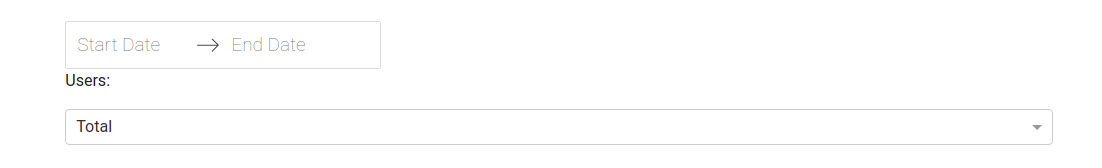
\includegraphics[width=16cm, keepaspectratio]{img/filtros.png}
    \caption{Filtros utilizados en Dash}
    \label{fig:filtros}
\end{figure}

Dash utiliza el modulo Plotly para generar las visualizaciones. Plotly ofrece una gran variedad de gráficas que se pueden utilizar en Dash. Adicionalmente se puede combinar varias gráficas en los mismos ejes, haciendo más sencilla la correlación entre datos. El código, por ejemplo, para crear la gráfica de número de sesiones por día es:\\
{\footnotesize
\begin{verbatim}
fig = px.line(df, x='start_date', y='count')
    fig.update_layout(xaxis_tick0=df['start_date'][0], xaxis_dtick=86400000 * 2)
    fig.add_trace(go.Scatter(x=df["start_date"].tolist(), y=df["count"].tolist(),
                             mode="markers", textposition="top center", 
                             name="Number of sessions",
                             text=df["count"].tolist()))
return fig
\end{verbatim}
}
\\
\newpage

\section{Validación experimental}

En esta sección se detallan los resultados finales de las analíticas con datos reales de la plataforma de Unibotics, donde se muestran las diferentes gráficas creadas tanto para administradores como para los usuarios, así como una explicación de lo que representan.\\

La primera gráfica creada se muestra en la Figura \ref{fig:sesion} , donde se representa en el eje x el tiempo y en el eje y el número de sesiones, dando como resultado una gráfica de linea con énfasis en los puntos para una mejor visualización. Esta gráfica muestra el número de sesiones por día. La gráfica muestra que días ha habido más \textit{logings}, viéndose en este ejemplo como en los meses de verano dicho número se ha reducido.



\begin{figure}[H]
    \centering
    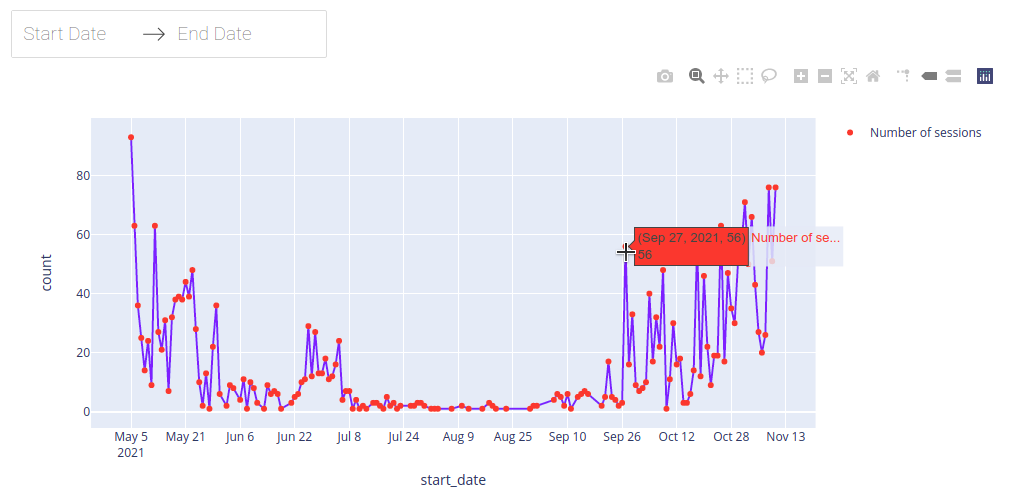
\includegraphics[width=18cm, keepaspectratio]{img/sesion.png}
    \caption{Gráfico sesiones totales por día}
    \label{fig:sesion}
\end{figure}
\newpage
En todas las gráficas de Dash si se pone el cursor sobre uno de los puntos se puede ver la información con mayor detalle, como se muestra en la Figura \ref{fig:sesion}. Igualmente Dash añade varias opciones para interactuar con la gráfica, por ejemplo, se puede descargar la gráfica, hacer \textit{zoom} o seleccionar una parte de ella. \\

Se ha creado otra gráfica lineal de sesiones por día, pero en este caso solo se tiene en cuenta el número de sesiones por usuario único. La gráfica esta creada de la misma manera que la gráfica del total de sesiones por día y con los mismos filtros (fechas y usuarios). En la Figura \ref{fig:sesion_users}  se muestra una parte ampliada de dicha gráfica.\\

\begin{figure}[H]
    \centering
    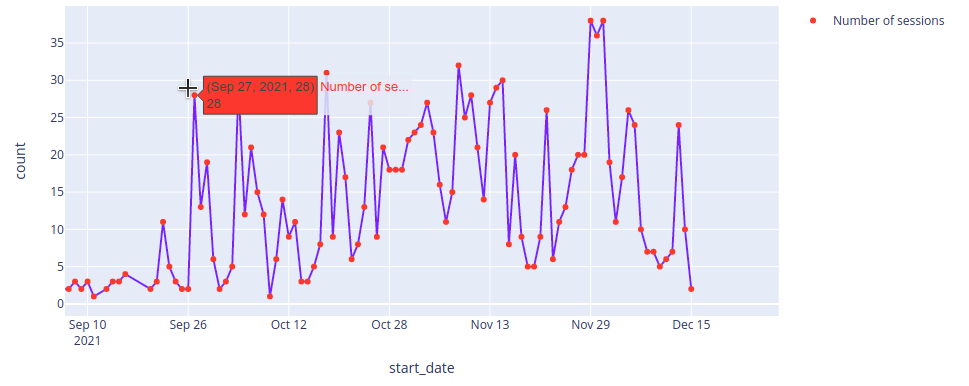
\includegraphics[width=18cm, keepaspectratio]{img/sesion_users.png}
    \caption{Gráfico sesiones únicas por día}
    \label{fig:sesion_users}
\end{figure}
\newpage
La Figura \ref{fig:time} muestra una gráfica de barras en la cual se representa el tiempo mediante el eje x y la duración total de la sesión de los usuarios en minutos en el eje y. Además, se ha incluido una media que representa la duración media de las sesiones. Aquí podemos comprobar que a veces la media coincide con la duración total debido a que solo ha tenido que haber una sesión en ese día.



\begin{figure}[H]
    \centering
    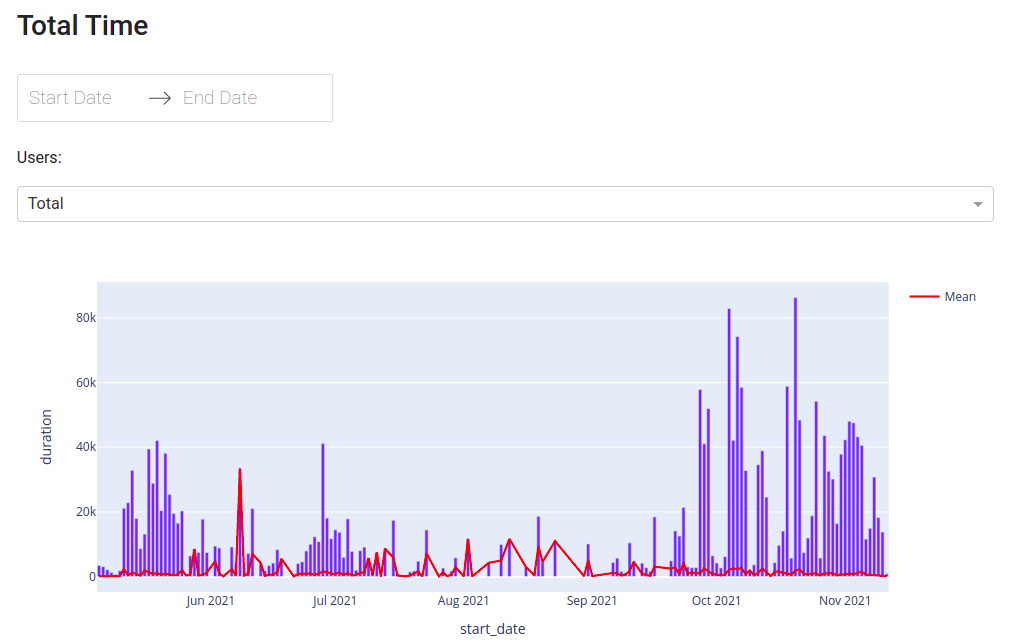
\includegraphics[width=18cm, keepaspectratio]{img/time.png}
    \caption{Gráfico de tiempo en Unibotics}
    \label{fig:time}
\end{figure}
Esta gráfica se puede filtrar tanto por fechas como por usuarios, pudiendo ver el tiempo dedicado de un usuario y la media total del tiempo que usa Unibotics dicho usuario, como se puede ver en la Figura \ref{fig:time_user}.

\begin{figure}[H]
    \centering
    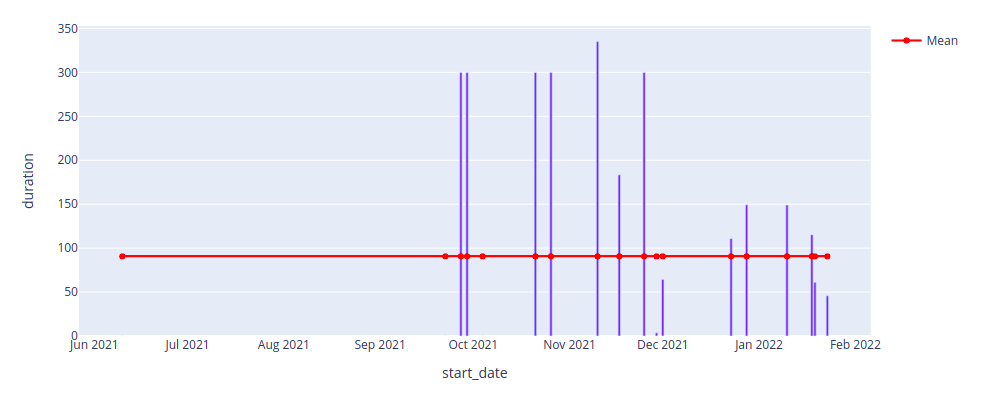
\includegraphics[width=18cm, keepaspectratio]{img/time_user.png}
    \caption{Gráfico de tiempo en Unibotics de un usuario}
    \label{fig:time_user}
\end{figure}
A fin de poder hacer un análisis de la media, la desviación típica o la moda se ha creado un histograma de las duraciones de las sesiones como se ve en la Figura \ref{fig:time_user}.
\begin{figure}[H]
    \centering
    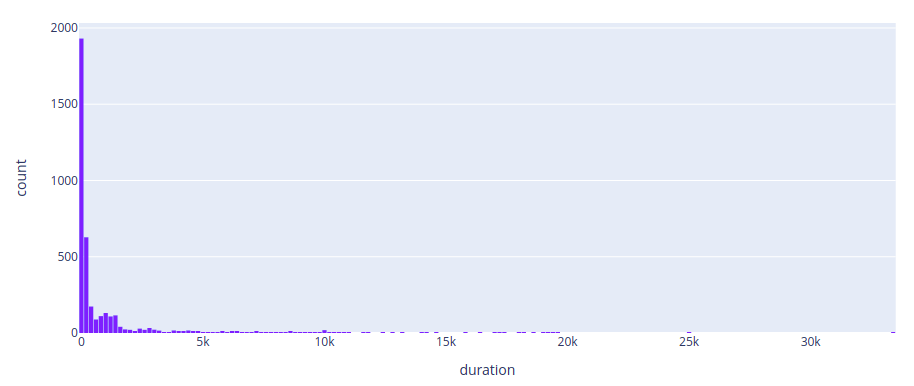
\includegraphics[width=16cm, keepaspectratio]{img/time_histogram.png}
    \caption{Histograma de las duraciones de sesiones}
    \label{fig:time_histogram}
\end{figure}
\newpage
La Figura \ref{fig:browser} muestra una gráfica con los distintos navegadores que utilizan los usuarios para acceder a Unibotics,  en formato porcentaje. En este caso se ve que una gran parte de inicio de sesiones es a través del navegador de Chrome.


\begin{figure}[H]
    \centering
    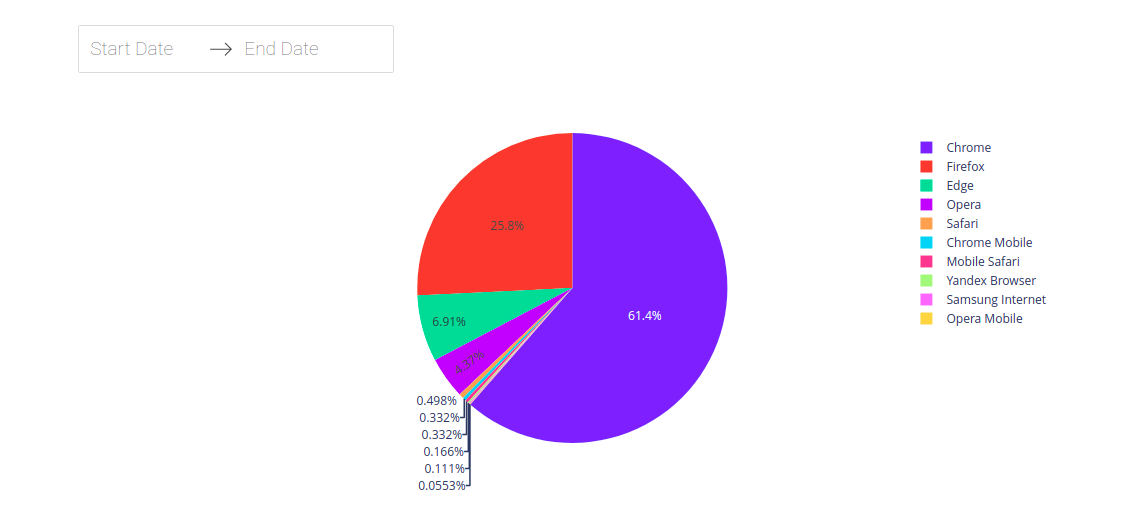
\includegraphics[width=19cm, keepaspectratio]{img/browser.png}
    \caption{Gráfico de navegadores}
    \label{fig:browser}
\end{figure}
\newpage
Se ha creado una gráfica similar a la anterior para representar los Sistemas Operativos utilizados por los usuarios que acceden a Unibotics, como se puede ver en la Figura \ref{fig:os}. Ambas gráficas tienen filtro por fechas.


\begin{figure}[H]
    \centering
    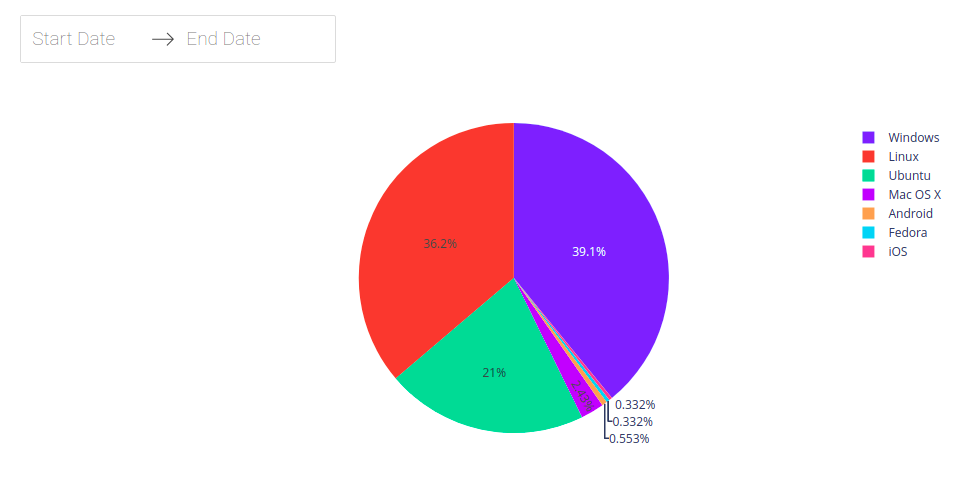
\includegraphics[width=17cm, keepaspectratio]{img/os.png}
    \caption{Gráfico de sistemas operativos}
    \label{fig:os}
\end{figure}
\newpage
En la Figura \ref{fig:mundo} se muestra un mapa geográfico con la localización de los usuarios que acceden a Unibotics. El tamaño de los puntos depende de la cantidad de sesiones, cuanto mayor sea el punto más sesiones hay. A la derecha se encuentra una leyenda con los países, se puede seleccionar uno o varios países en la leyenda para que solo se vean ellos en el mapa. Se puede filtrar por fechas.



\begin{figure}[H]
    \centering
    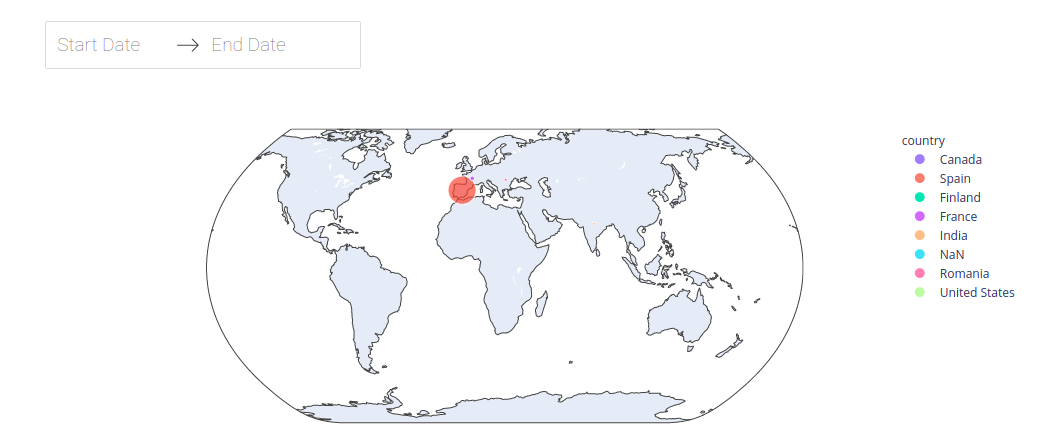
\includegraphics[width=17cm, keepaspectratio]{img/mundo.png}
    \caption{Mapa geográfico de sesiones}
    \label{fig:mundo}
\end{figure}
\newpage
En la siguiente gráfica que se ve en la Figura \ref{fig:activity} representa un mapa de calor con la actividad de los usuarios. Esta dividido en cuadrados que representan cada día de un año, cuanto más intenso es el color verde más sesiones ha habido, ha medida que disminuyen las sesiones la intensidad también baja. A parte del filtrado por fechas. tiene un filtro por usuario para ver la actividad por usuarios únicos o grupo de ellos. Como ocurría con la gráfica lineal de sesiones, el primer mapa de color cuenta el total de las sesiones y el segundo mapa de color cuenta las sesiones únicas por usuario.


\begin{figure}[H]
    \centering
    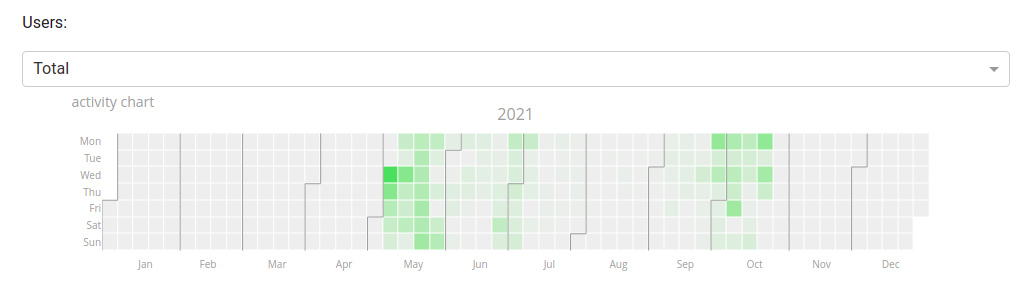
\includegraphics[width=17cm, keepaspectratio]{img/activity.png}
    \caption{Mapas de calor sesiones}
    \label{fig:activity}
\end{figure}
\newpage

Los administradores tienen la opción de poder ver el número total de usuarios que son activos, el número de usuarios que han sido activos en los últimos 2 meses, en formato número. Además se muestra las gráficas de linea de registros por cada día, registros acumulados por días (Figura \ref{fig:accumulated}) y usuarios activos en los últimos 2 meses.(Figura \ref{fig:active}) Cada día se comprueba cuantos usuarios han iniciado sesión desde 2 meses atrás hasta ese día concretamente. Cada una de estas gráficas contiene su propio filtrado por fechas. 

\begin{figure}[H]
    \centering
    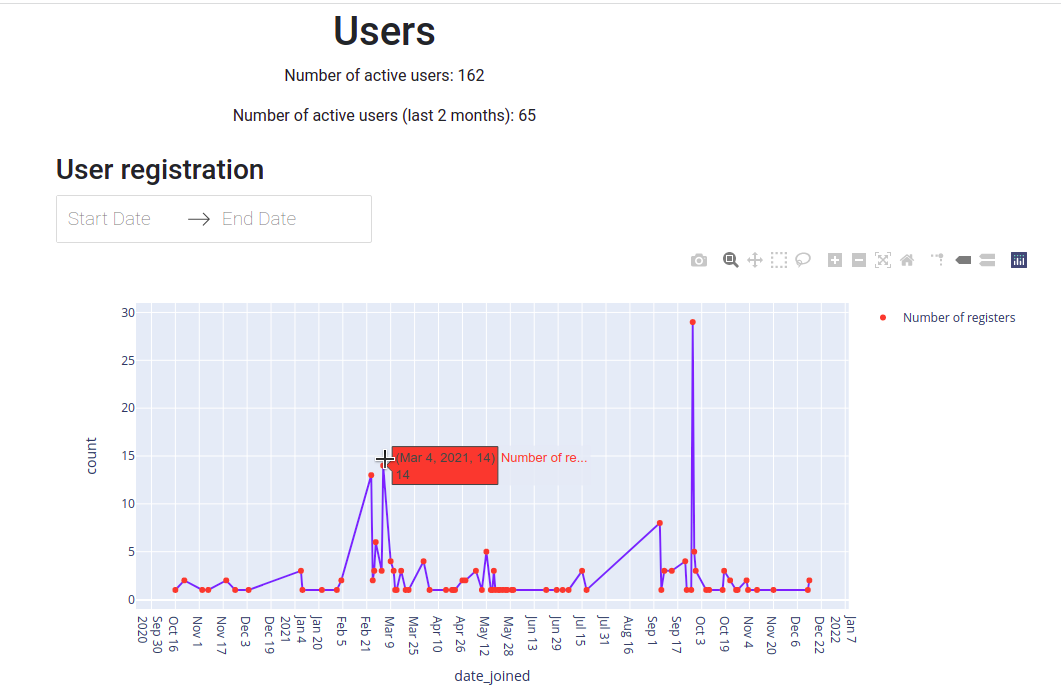
\includegraphics[width=17cm, keepaspectratio]{img/users.png}
    \caption{Gráficas relativas a los usuarios}
    \label{fig:users}
\end{figure}
\begin{figure}[H]
    \centering
    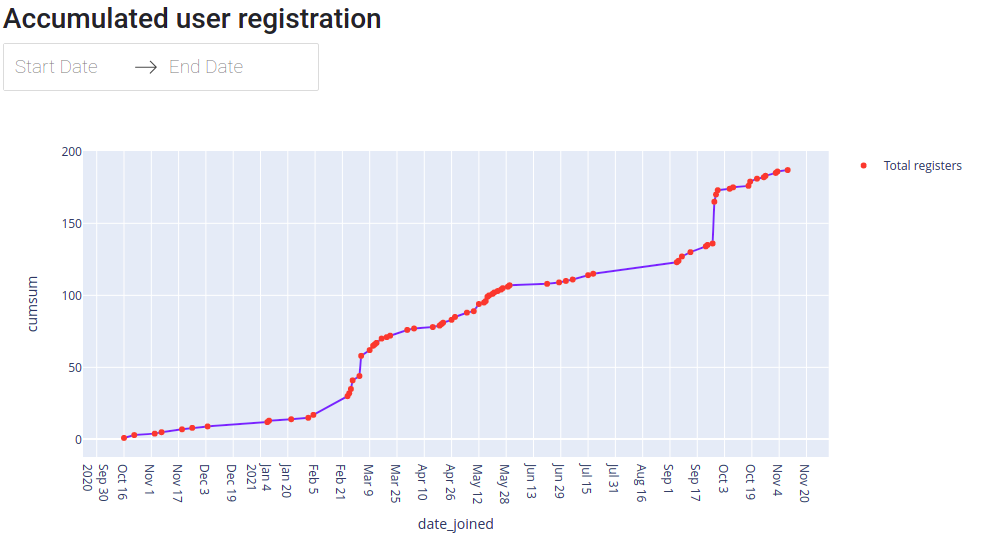
\includegraphics[width=17cm, keepaspectratio]{img/accumulated.png}
    \caption{Gráfica registro de usuarios acumulado}
    \label{fig:accumulated}
\end{figure}
\begin{figure}[H]
    \centering
    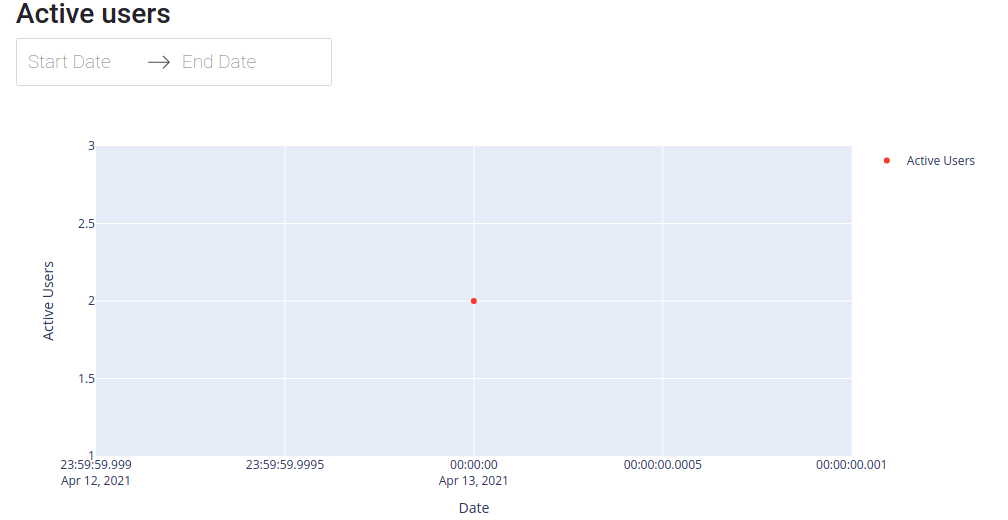
\includegraphics[width=17cm, keepaspectratio]{img/active.png}
    \caption{Gráfica de usuarios activos cada día}
    \label{fig:active}
\end{figure}
\newpage
Con el propósito de conocer el tiempo que invierten los usuarios en cada ejercicio se ha elaborado un histograma de las duraciones de los ejercicios. Esta gráfica dispone de un filtro del ejercicio que se desea comprobar, con el filtro de usuario y el de fechas. Por ejemplo, la Figura \ref{fig:histogram_exercise} es un histograma del ejercicio \textit{follow\_line}  de un grupo de usuarios y unas fechas concretas.
\begin{figure}[H]
    \centering
    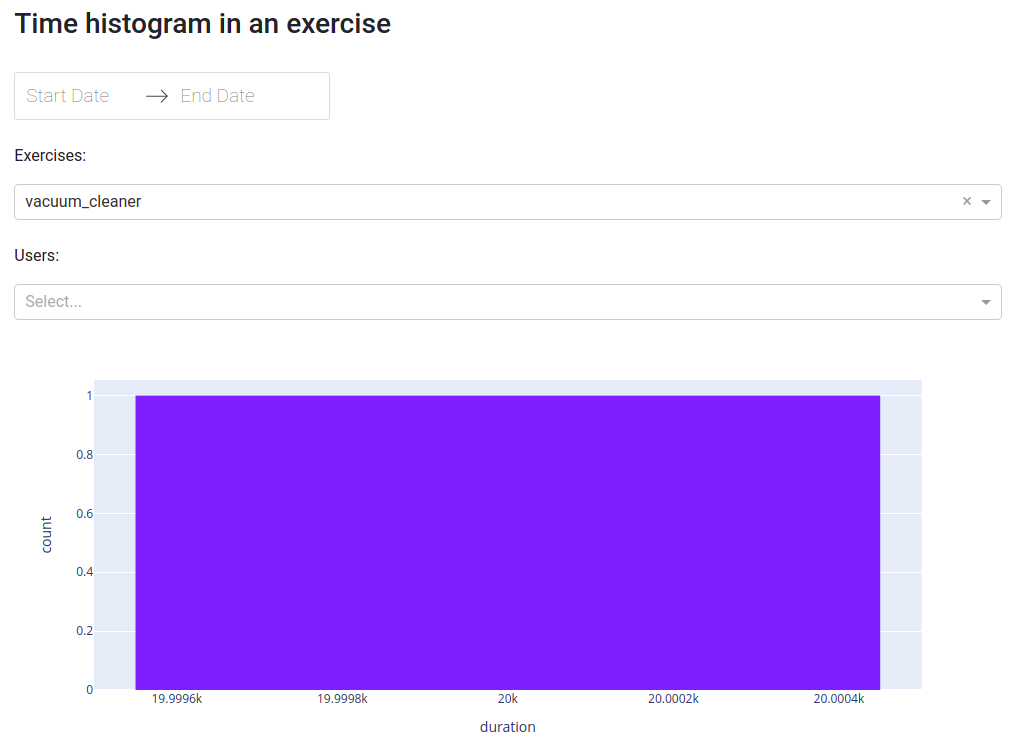
\includegraphics[width=17cm, keepaspectratio]{img/histogram_exercise.png}
    \caption{Histograma del ejercicio follow\_line de un grupo de usuarios }
    \label{fig:histogram_exercise}
\end{figure}
\newpage

Las siguientes gráficas son las puntuaciones de estilo y eficacia que podrán ser vistas tanto por los usuarios (que pueden acceder a sus puntuaciones) como por los administradores (que pueden acceder a las puntuaciones de todos los usuarios).  Actualmente las evaluaciones solo están disponibles en cuatro ejercicios representadas en una gráfica, en la que cada punto es una evaluación solicitada por el usuario. Las gráficas mostradas en las Figuras \ref{fig:score} y \ref{fig:score_efficacy}  son un ejemplo de las notas de estilo y eficacia de un usuario de la base de datos de prueba en el ejercicio \textit{follow\_line}. Las gráficas de los demás ejercicios son iguales. como las de las puntuaciones de eficacia.



\begin{figure}[H]
    \centering
    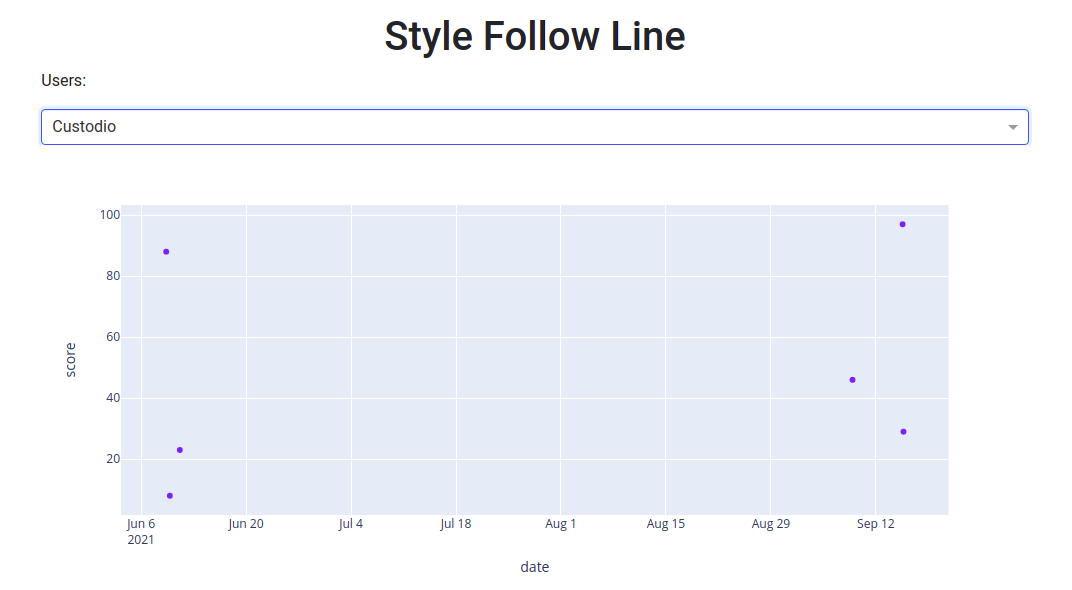
\includegraphics[width=17cm, keepaspectratio]{img/score.png}
    \caption{Gráfica de puntuación de estilo}
    \label{fig:score}
\end{figure}


\begin{figure}[H]
    \centering
    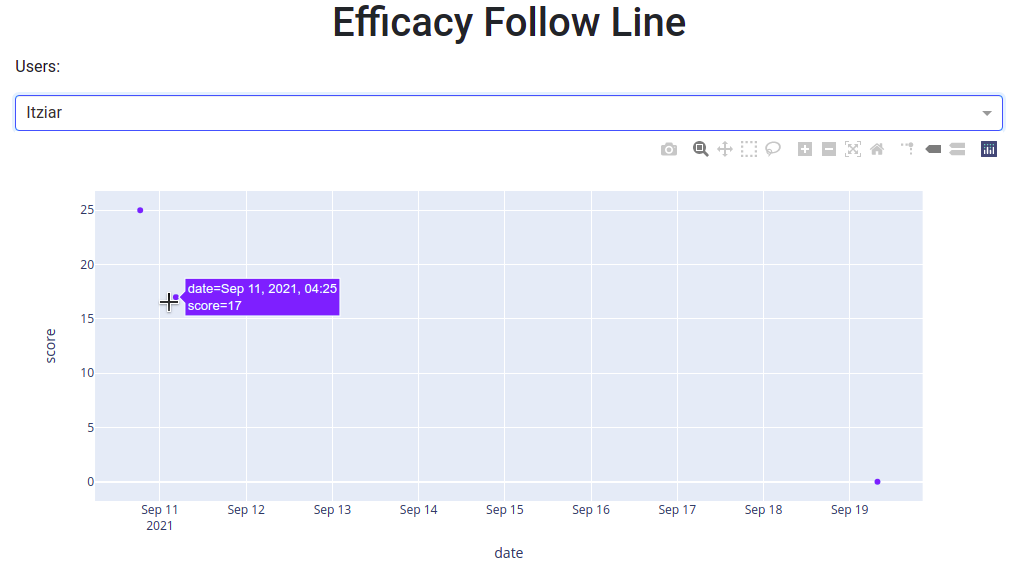
\includegraphics[width=17cm, keepaspectratio]{img/score_efficacy.png}
    \caption{Gráfica de puntuación de eficacia}
    \label{fig:score_efficacy}
\end{figure}









